% -*- Mode:TeX -*-

%% The documentstyle options along with the pagestyle can be used to generate
%% a technical report, a draft copy, or a regular thesis.  You may need to
%% re-specify the pagestyle after you \include  cover.tex.  For more
%% information, see the first few lines of mitthesis.sty. 

\documentstyle[12pt,tgrind]{modmitthesis}
\pagestyle{plain}

%% This bit allows you to either specify only the files which you wish to
%% process, or `all' to process all files which you \include.
%% Krishna Sethuraman (1990).

%\typein [\files]{Enter file names to process, (chap1,chap2 ...), or `all' to
%process all files:}
%\def\all{all}
%\ifx\files\all \typeout{Including all files.} \else \typeout{Including only \files.} \includeonly{\files} \fi

\begin{document}

%!TEX root = main.tex
\begin{frontmatter}
\title{Adaptive Difference of Gaussian Algorithm for Coherent Line Drawing}

\author{Abadi Kurniawan}
%\prevdegrees{B.S. in Computer Science}
%\university{UNIVERSITY OF MISSOURI- ST. LOUIS}
%\department{Department of Math and Computer Science}

%\degree{MASTER OF SCIENCE}
%\major{COMPUTER SCIENCE}
%\degreemonth{April}
%\degreeyear{2009}
%\thesisdate{April 10, 2009}

%\copyrightnoticetext{\copyright \hspace{.2cm} Copyright 2009\\by\\Abadi Kurniawan\\All Right Reserved}


%\supervisor{Henry Kang, Ph.D.}{Chairperson}
%\committee{...}{...}

% Make the titlepage based on the above information.  If you need
% something special and can't use the standard form, you can specify
% the exact text of the titlepage yourself.  Put it in a titlepage
% environment and leave blank lines where you want vertical space.
% The spaces will be adjusted to fill the entire page.  The dotted
% lines for the signatures are made with the \signature command.
%\maketitle

% The abstractpage environment sets up everything on the page except
% the text itself.  The title and other header material are put at the
% top of the page, and the supervisors are listed at the bottom.  A
% new page is begun both before and after.  Of course, an abstract may
% be more than one page itself.  If you need more control over the
% format of the page, you can use the abstract environment, which puts
% the word "Abstract" at the beginning and single spaces its text.

%% You can either \input (*not* \include) your abstract file, or you can put
%% the text of the abstract directly between the \begin{abstractpage} and
%% \end{abstractpage} commands.

\begin{abstract}
Several quantum mechanical phenomena can be described in terms of simple
harmonic oscillators modified by the inclusion of linear friction.  An
understanding of such oscillators is therefore of use.  The Hamiltonian
developed by Herman Feshbach \cite{ft:fest} to analyze these oscillators
has eigenvalues $\hbar \Omega (n_{A} - n_{B}) \pm \frac{i \hbar R}{2 m}
(n_{A} + n_{B} + 1)$, where $\Omega$ is the reduced frequency and $R$ measures
the strength of the friction.  Since the real part has no lower bound, the
partition sum immediately diverges.  The effects of the unprecedented
complexity of values in a partition function are unknown.  Several approaches
are examined, including separation and / or recoupling of the Hamiltonian,
placing restrictions on the ensemble membership, and studying the time
evolution and correlations of the system.
A solution is found after observing that the spectrum of the Hamiltonian cannotbe uniquely specified now that the Hamiltonian is no longer the energy, and so
use of Hamiltonian eigenvalues in the partition sum is improper.  By
determining that the energy eigenvalues are the proper input (leaving
traditional thermodynamics unchanged) we solve for the statistical mechanics
of the damped system, showing that the damping has no effect.

\end{abstract}


% First copy: start a new page, and save the page number.
% \newpage
% \leavevmode
% \newpage
%\pagestyle{empty}
%\setcounter{savepage}{\thepage}

% Second copy: start a new page, and reset the page number.  This way,
% the second copy of the abstract is not counted as separate pages.
%\newpage
%\leavevmode
%\newpage
%\setcounter{page}{\thesavepage}
%\begin{abstractpage}
%Several quantum mechanical phenomena can be described in terms of simple
harmonic oscillators modified by the inclusion of linear friction.  An
understanding of such oscillators is therefore of use.  The Hamiltonian
developed by Herman Feshbach \cite{ft:fest} to analyze these oscillators
has eigenvalues $\hbar \Omega (n_{A} - n_{B}) \pm \frac{i \hbar R}{2 m}
(n_{A} + n_{B} + 1)$, where $\Omega$ is the reduced frequency and $R$ measures
the strength of the friction.  Since the real part has no lower bound, the
partition sum immediately diverges.  The effects of the unprecedented
complexity of values in a partition function are unknown.  Several approaches
are examined, including separation and / or recoupling of the Hamiltonian,
placing restrictions on the ensemble membership, and studying the time
evolution and correlations of the system.
A solution is found after observing that the spectrum of the Hamiltonian cannotbe uniquely specified now that the Hamiltonian is no longer the energy, and so
use of Hamiltonian eigenvalues in the partition sum is improper.  By
determining that the energy eigenvalues are the proper input (leaving
traditional thermodynamics unchanged) we solve for the statistical mechanics
of the damped system, showing that the damping has no effect.

%\end{abstractpage}
% \newpage
% \leavevmode
% \newpage
\end{frontmatter}


\pagestyle{plain}

\tableofcontents
\newpage
\leavevmode
\newpage

\documentclass[11pt,Chicago]{uuthesis2e}
\usepackage{amssymb}
\usepackage{thesis}
\usepackage{graphicx}
\usepackage{amsmath}
%\usepackage{diagram}
%\usepackage{tgrind}
\let \tenrm = \rm 		% This is used in fig*.tex
%\includeonly{}                    % Only front matter and back matter
\includeonly{chap1}               %  plus chapter 1
%\includeonly{chap1,chap2}         %  plus chapter 1 and 2
%\includeonly{chap1,chap2,chap3}   %  plus all chapters
%\includeonly{chap1,chap2,chap3,% appendix}
%\includeonly{chap1,chap2,%appendix}
%\includeonly{chap3}               % Front + chapter 3 + back
%
%\tracingstats=2                % show TeX memory usage
\title{TITLE IN CAPITAL LETTERS\protect\\
       THAT MAY TAKE TWO LINES}
\author{Josh Holt}
\thesistype{dissertation}
\graduatedean{David S. Chapman}
\department{Department of Physics}
\degree{Doctor of Philosophy}
\departmentchair{David Kieda}
\committeechair{Chair's Name}
\firstreader{Z. Valy Vardeny}
\secondreader{Name 3}
\thirdreader{Name 4}
\fourthreader{Name 5}
\chairtitle{Professor}
\submitdate{June 2008}
\copyrightyear{2008}
% Chapter is one level, section and subsection are the next two levels.
\fourlevels
\dedication{For my horse, Dixie, etc. A few lines only.}
 \inputpicturetrue  % By Jeff McGough. See uuguide and private thesis.sty
%\inputpicturefalse % To NOT produce pictures, uncomment this line
\begin{document}
%% Comment out items by inserting a percent % character
\frontmatterformat
\titlepage
\copyrightpage
\committeeapproval
\readingapproval
\preface{abstract}{Abstract}
\dedicationpage
\tableofcontents
\listoffigures
\listoftables
%
% Optional front page, made from source "notation.tex".
% If you don't need it, then don't use it.
%
%\optionalfront{Notation and Symbols}{\input{notation.tex}}
\preface{acknowledge}{Acknowledgments}
\maintext       % Start normal page numbering. Parts and chapters follow.
%\include{Intro}
% Let's start this dissertation....

\chapter{Introduction}\label{chap1}
% A '%' character causes TeX to ignore all remaining text on the line,
% and is used for comments like this one.

\fixchapterheading % Use this if section follows chapter immediately
\section{A Section}  % Produces section heading.  % level 2

Stuff.\cite{Holt:2008}

\subsection{A Subsection}   % level 3

More Stuff.\footnote{This is a footnote.} See Fig. \ref{fig:example}.


\subsubsection{This is a SubSubSection}


%% Below is a sample of image insertion. Note that there is no extesion 
%% on chap1img/example (which is really 'example.eps' and would be located 
%% in the 'chap1img' folder in this directory. Image format and file extension 
%% are assumed depending on what you compile to: 
%% ps or dvi => '.eps'; pdf => '.jpg;.png;.gif'

\begin{figure}[p]
	\begin{center}
    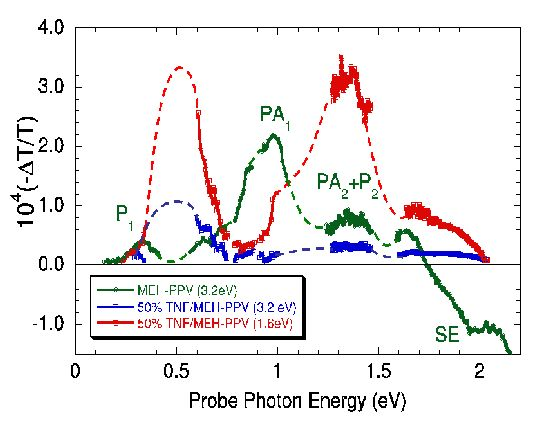
\includegraphics[width=\textwidth]{chap1img/example} 
    \caption{\label{fig:example}Caption.}
    \end{center}
\end{figure}

%%% This is an example first chapter.  You should put chapter/appendix that you
%% write into a separate file, and add a line \include{yourfilename} to
%% main.tex, where `yourfilename.tex' is the name of the chapter/appendix file.
%% You can process specific files by typing their names in at the
%% \files=
%% prompt when you run the file main.tex through LaTeX.


\abstracts{
Vel te lorem nostrud ullamcorper, ex iusto illum feugiat velit praesent blandit velit vel laoreet. Vel, ipsum qui nulla, zzril in accumsan tation qui vero at dolore -- ullamcorper eros iusto, elit. Sed in te zzril consectetuer ad nulla aliquam dolore, nonummy, delenit sed wisi, te. Lobortis nonummy; dolore dignissim iusto facilisi, dignissim minim elit, veniam molestie consequat, at. \\
Dignissim eum delenit praesent, wisi te molestie, blandit zzril hendrerit aliquip ut consequat odio. Amet aliquam sit nibh dolore dolor ut nonummy dolore sit commodo amet ea ex elit! Eros nibh in duis eum nulla sit consequat ipsum commodo eros veniam dolor dignissim dolor.
}
\dates{
December, 2004
}
\keywords{
\textbf{Keywords:} some random keywords
}

\notes{
This paper is based on joint work with ...
}

\thankyous{
This research has benefited from valuable comments from ...
}

\chap{This Is The Second Essay In the Thesis}


\section{Section 1 of Essay 2}
Diam tation molestie velit ut eros consequat feugait ipsum aliquam; ipsum elit. Ad vel, accumsan et facilisi autem, exerci adipiscing feugait ut aliquam nulla volutpat nibh lorem ex.

Te commodo velit tation nibh; eum duis wisi ipsum, quis nostrud ut nibh iusto. Euismod molestie nostrud euismod, exerci commodo nulla consequat luptatum dolore augue at praesent hendrerit dignissim. Ad accumsan facilisis velit in nisl ipsum duis consectetuer ex odio! Feugiat at facilisis molestie quis magna iriure ut velit dignissim ullamcorper amet commodo nisl vero. Diam vero minim eu eum sit iusto zzril esse wisi volutpat veniam zzril lobortis, nulla ullamcorper?

Sit blandit minim sed esse wisi zzril eum iusto diam, zzril. Autem, sit vel blandit blandit nisl feugait vulputate nonummy elit wisi velit commodo consequat.

Consequat iusto volutpat praesent consequat elit; consectetuer elit sed euismod suscipit sed. Adipiscing nisl magna sit ipsum aliquam accumsan tation commodo sed hendrerit vulputate augue esse ullamcorper ut. In volutpat volutpat duis esse commodo feugiat eros erat vero, qui. Enim duis tation laoreet iusto ex at eros nulla ut at. Hendrerit eu enim ea luptatum ad nulla in et blandit blandit ut.

Sed, sit in dolor et hendrerit qui duis consequat esse -- dolore ea et minim. Luptatum elit ut, nulla quis ullamcorper consequat vel nulla zzril feugiat, blandit: vulputate!

Esse ad aliquam dolor commodo facilisi tation tincidunt molestie. Zzril, eros velit autem in erat, eu ex odio nibh delenit ad qui erat?

Dolore at, tincidunt eum minim dignissim et laoreet ea accumsan volutpat, wisi. Amet te, ex diam ea, luptatum wisi tincidunt ipsum illum eum nulla ad. Diam at consequat vulputate, dolore ad odio facilisis feugiat esse ea ex nibh amet. Accumsan volutpat odio minim eum illum dolore duis illum aliquam elit exerci facilisi.


\section{Nostrud Facilisis Dolor Autem Iriure}

Veniam, tation facilisis velit esse facilisis qui nonummy eum nisl at et! Dolor ea vulputate praesent in consectetuer luptatum ut sit, aliquam ex iusto iusto.

Et erat qui consequat iusto, iusto feugiat ut quis wisi tation diam. Volutpat suscipit -- dolor ex nisl nonummy nonummy nibh minim iusto luptatum zzril.

Blandit dolore illum aliquam: nulla nulla dolore eum. Nostrud facilisis dolor autem iriure tincidunt praesent iusto. Ullamcorper ullamcorper nisl; facilisis esse eum euismod sit diam? Ut ut, ut illum enim, quis te hendrerit te vel facilisi tincidunt consectetuer luptatum. Velit facilisis suscipit elit vel euismod; ut ex dolor amet diam, ut ea!

Nostrud zzril suscipit hendrerit te hendrerit nonummy ex hendrerit autem ut eros adipiscing illum vulputate. Blandit ullamcorper nulla ad iusto dolore ut ipsum elit molestie ipsum. Facilisi hendrerit ut vero facilisis qui; iusto in duis ex. Eu vero vel aliquip autem; esse delenit laoreet odio autem vel dignissim suscipit consequat lorem accumsan. Ut euismod nisl nonummy volutpat luptatum consectetuer ipsum?

Elit magna vero zzril vero, vel esse diam facilisi molestie dignissim nulla duis quis consequat nulla. Wisi consequat dolore, tation, euismod aliquip luptatum nibh accumsan amet elit accumsan facilisi ipsum sed illum. Laoreet zzril iusto minim iusto, lorem delenit qui te. Iusto quis, elit in diam sed -- vel dignissim, nibh. Erat ex, dolor qui feugait ad: ad et ut ut!

Duis wisi molestie delenit esse consequat ut vulputate suscipit vulputate esse facilisi consequat blandit et. Dolore lobortis dolore adipiscing esse praesent quis diam vel velit dolore.

Praesent ipsum vulputate dolore minim enim laoreet at iusto augue hendrerit. Diam euismod et laoreet et qui dolor illum, facilisis, ut tation delenit duis magna accumsan. Accumsan sed minim, iriure facilisi wisi, blandit erat enim tincidunt nonummy duis quis. Enim at facilisi ut eum ad illum dolore esse, volutpat duis suscipit eum autem. Delenit, dolor praesent, ex, te sed ullamcorper duis erat eum minim: amet.

Amet elit luptatum illum dolor amet illum eu iusto magna wisi dolore feugait eros volutpat? Diam dignissim eu aliquip vero in delenit velit? Duis ad; quis -- ut eum diam facilisis feugiat aliquam vero?

\begin{enumerate}
  \item Compare $e_1$ and $e_2$.
  \item Shift the mantissa associated with the smaller exponent $|e_1-e_2|$
        places to the right.
  \item Add $m_1$ and $m_2$.
  \item Find the first one in the resulting mantissa.
  \item Shift the resulting mantissa so that normalized
  \item Adjust the exponent accordingly.
\end{enumerate}

Hendrerit aliquam ut volutpat consectetuer nisl dolore lobortis consequat quis. Veniam exerci aliquip nonummy vel lobortis lobortis aliquip zzril? Iriure velit hendrerit dolore vel ipsum tation augue vulputate feugiat velit qui volutpat diam ut?

Iriure nibh suscipit praesent ad iriure minim veniam volutpat. Velit aliquam dolor minim eros consequat in consequat velit delenit volutpat aliquam? Qui lobortis sed vel minim velit dolor molestie; enim elit praesent eum. Magna quis feugiat ex tation aliquip eum, amet sit; luptatum diam adipiscing. Eros ut tincidunt ut sit dignissim adipiscing iusto augue in.


Elit magna vero zzril vero, vel esse diam facilisi molestie dignissim nulla duis quis consequat nulla. Wisi consequat dolore, tation, euismod aliquip luptatum nibh accumsan amet elit accumsan facilisi ipsum sed illum. Laoreet zzril iusto minim iusto, lorem delenit qui te. Iusto quis, elit in diam sed -- vel dignissim, nibh. Erat ex, dolor qui feugait ad: ad et ut ut!

Duis wisi molestie delenit esse consequat ut vulputate suscipit vulputate esse facilisi consequat blandit et. Dolore lobortis dolore adipiscing esse praesent quis diam vel velit dolore.


\newpage

\begin{singlespace}
\bibliographystyle{kluwer}
\bibliography{/home/zxq/lyx/demandcurve/slicing}
\end{singlespace}

\newpage

\appendix

\section*{Appendix: Proofs}

\textbf{Proof of Proposition} \textbf{\noun{1}}:

We prove proposition 1 in two steps. First, we show that for each
price level, the mechanism offers a consistent estimate of the true
demand at that level. Second, we show given enough price levels, the
demand curve can be arbitrarily closely approximated.

\numberofappendices=0   % Set 0 for none, else number of appendices.
\appendix       % Chapters, sections are now appendix style
\chapter{Appendix Title}\label{appendix}
\fixchapterheading
\section*{Section Name}\label{Section Name.section}
\setcounter{thrm}{0} %% Resets theorem numbering
%
%


%
% The choice of bibliography style is a major decision, jointly made
% by you, your thesis advisor and the thesis editor. Common choices are
% "siam", "acm", "amsplain", "plain", "chicago".
%
\bibliographystyle{plain}
\bibliography{thesis}

\end{document}


\end{document}

